\documentclass{article}

\usepackage{microtype}
\usepackage{amsmath}
\usepackage{enumitem}
\usepackage{etoolbox}
% \usepackage{pgfplots}
\usepackage[svgnames]{xcolor}
\usepackage{tikz}
\usepackage{tikz-3dplot}
\usepackage[letterpaper, bottom=100pt]{geometry}
\usepackage{physics}
\usepackage{float}

% \pgfplotsset{compat=newest}

\newcommand{\diff}[1]{\frac{#1}{dt}}
\newcommand{\vel}{\mathrm{v}}
\newcommand{\x}{\mathrm{x}}
\newcommand{\inter}{\int_{t_1}^{t_2}}
\newcommand{\tvert}{\biggr\rvert_{t_1}^{t_2}}
\newcommand{\derv}{\frac{\mathrm{d}}{\mathrm{d}t}}

\patchcmd\subequations
 {\theparentequation\alph{equation}}
 {\subequationsformat}
 {}{}

\newcommand{\subequationsformat}{\theparentequation.\arabic{equation}}

\author{Laith}
\title{Vectors and 3-Dimensional Space}
\date{1/30/2023}

\begin{document}
\maketitle
\section{Visualizing a 3D Space}
Objects can move in 3 ways with respect to a position, and \textbf{vectors} are used to
represent this. Vectors include both a direction and a distance.
\begin{figure}[H]
\begin{center}
\begin{tikzpicture}
\tdplotsetmaincoords{60}{110};
\pgfsetxvec{\pgfpoint{0.866cm}{-.5cm}};
\pgfsetyvec{\pgfpoint{0cm}{1cm}};
\pgfsetzvec{\pgfpoint{-.866cm}{-.5cm}};

\draw[->, color=green] (0, 0, 0) -- (3, 0, 0) node[anchor=west] {X};
\draw[->, color=blue] (0, 0, 0) -- (0, 3, 0) node[anchor=south] {Y};
\draw[->, color=red] (0, 0, 0) -- (0, 0, 3) node[anchor=north east] {Z};
\end{tikzpicture}
\end{center}
\end{figure}

If we take the gray lines in the figure below:
\begin{figure}[H]
\begin{center}
\begin{tikzpicture}[scale=0.75]
\tdplotsetmaincoords{60}{110};
\pgfsetxvec{\pgfpoint{0.866cm}{-.5cm}};
\pgfsetyvec{\pgfpoint{0cm}{1cm}};
\pgfsetzvec{\pgfpoint{-.866cm}{-.5cm}};

\draw[->, color=green] (0, 0, 0) -- (3, 0, 0) node[anchor=west] {X};
\draw[->, color=blue] (0, 0, 0) -- (0, 3, 0) node[anchor=south] {Y};
\draw[->, color=red] (0, 0, 0) -- (0, 0, 3) node[anchor=north east] {Z};

\draw[->, color=black] (0, 0, 0) -- (1, 4, 0) node (a) {};
\draw[->, color=black] (0, 0, 0) -- (-1, 4, 0) node (b) {};
\draw[<->, color=gray] (a) -- (b) node[above] {$\Delta x$};

\draw[->, color=black] (0, 0, 0) -- (4, 1, 0) node (a) {};
\draw[->, color=black] (0, 0, 0) -- (4, -1, 0) node (b) {};
\draw[<->, color=gray] (a) -- (b) node[right] {$\Delta y$};

\draw[->] (0, 0, 0) -- (-4, 0, -1) node (a) {};
\draw[->] (0, 0, 0) -- (-4, 0, 1) node (b) {};
\draw[<->, color=gray] (a) -- (b) node[above, yshift=3] {$\Delta z$};
\end{tikzpicture}
\end{center}
\end{figure}

and assign each of them a direction:
\begin{figure}[H]
\begin{center}
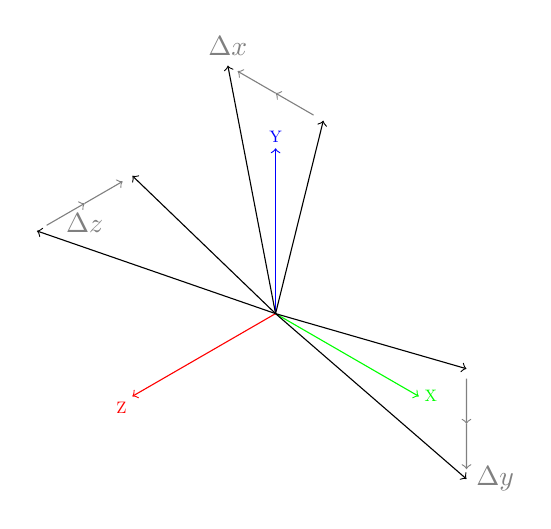
\begin{tikzpicture}[scale=0.7]
\tdplotsetmaincoords{60}{110};
\pgfsetxvec{\pgfpoint{0.866cm}{-.5cm}};
\pgfsetyvec{\pgfpoint{0cm}{1cm}};
\pgfsetzvec{\pgfpoint{-.866cm}{-.5cm}};

\draw[->, color=green] (0, 0, 0) -- (3, 0, 0) node[scale=0.6, anchor=west] {X};
\draw[->, color=blue] (0, 0, 0) -- (0, 3, 0) node[scale=0.6, anchor=south] {Y};
\draw[->, color=red] (0, 0, 0) -- (0, 0, 3) node[scale=0.6, anchor=north east] {Z};

\draw[->, color=black] (0, 0, 0) -- (4, 1, 0) node (a) {};
\draw[->, color=black] (0, 0, 0) -- (4, -1, 0) node (b) {};
\draw[->, color=gray] (a) -- (4, 0, 0);
\draw[->, color=gray] (4, 0, 0) -- (b) node[right] {$\Delta y$};

\draw[->, color=black] (0, 0, 0) -- (1, 4, 0) node (a) {};
\draw[->, color=black] (0, 0, 0) -- (-1, 4, 0) node (b) {};
\draw[->, color=gray] (a) -- (0, 4, 0);
\draw[->, color=gray] (0, 4, 0) -- (b) node[above] {$\Delta x$};

\draw[->] (0, 0, 0) -- (-4, 0, 1) node (a) {};
\draw[->] (0, 0, 0) -- (-4, 0, -1) node (b) {};
\draw[->, color=gray] (a) -- (-4, 0, 0) node[below] {$\Delta z$};
\draw[->, color=gray] (-4, 0, 0) -- (b);
\end{tikzpicture}
\end{center}
\end{figure}

We now have vectors! 
\section{Vectors}
Mathematically, vectors are represented as a variable
with an arrow on-top of it:
\[\va{a}\]
Above, we have a vector named \textbf{a}. This vector has various components:
\begin{align*}
    & \textbf{a} = \text{magnitude (distance)} \\
    & \textbf{a}_x = \text{x distance} \\
    & \textbf{a}_y = \text{y distance} \\
    & \textbf{a}_z = \text{z distance}
\end{align*}
Lets label our figure from before with vectors:
\begin{figure}[H]
\begin{center}
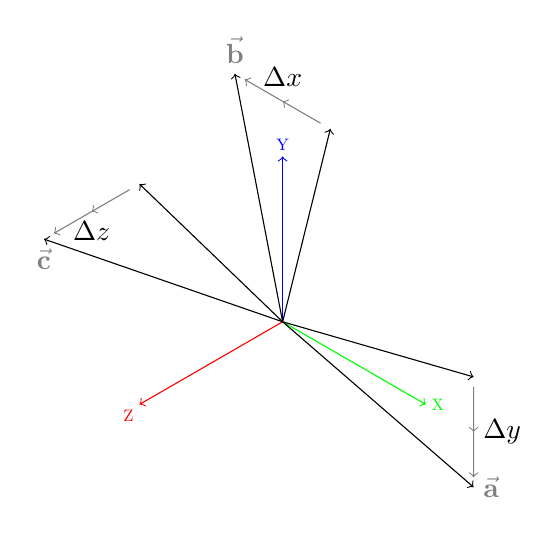
\begin{tikzpicture}[scale=0.7]
\tdplotsetmaincoords{60}{110};
\pgfsetxvec{\pgfpoint{0.866cm}{-.5cm}};
\pgfsetyvec{\pgfpoint{0cm}{1cm}};
\pgfsetzvec{\pgfpoint{-.866cm}{-.5cm}};

\draw[->, color=green] (0, 0, 0) -- (3, 0, 0) node[scale=0.6, anchor=west] {X};
\draw[->, color=blue] (0, 0, 0) -- (0, 3, 0) node[scale=0.6, anchor=south] {Y};
\draw[->, color=red] (0, 0, 0) -- (0, 0, 3) node[scale=0.6, anchor=north east] {Z};

\draw[->, color=black] (0, 0, 0) -- (4, 1, 0) node (a) {};
\draw[->, color=black] (0, 0, 0) -- (4, -1, 0) node (b) {};
\draw[->, color=gray] (a) -- (4, 0, 0);
\draw[->, color=gray] (4, 0, 0) node[color=black, right] {$\Delta y$} -- (b) node[right] {$\va{a}$};

\draw[->, color=black] (0, 0, 0) -- (1, 4, 0) node (a) {};
\draw[->, color=black] (0, 0, 0) -- (-1, 4, 0) node (b) {};
\draw[->, color=gray] (a) -- (0, 4, 0);
\draw[->, color=gray] (0, 4, 0) node[color=black, above, yshift=2] {$\Delta x$} -- (b) node[above] {$\va{b}$};

\draw[->] (0, 0, 0) -- (-4, 0, -1) node (a) {};
\draw[->] (0, 0, 0) -- (-4, 0, 1) node (b) {};
\draw[->, color=gray] (a) -- (-4, 0, 0);
\draw[->, color=gray] (-4, 0, 0) node[color=black, below] {$\Delta z$} -- (b) node[below] {$\va{c}$};
\end{tikzpicture}
\end{center}
\end{figure}

We can say that:
\begin{align*}
    \va{a} &= \Delta y \\
    \va{b} &= \Delta x \\
    \va{c} &= \Delta z 
\end{align*}
These vectors would be known as \textbf{displacement vectors}, which are the simplest type
of vectors and thus make for a good introductary example.
\end{document}